% Options for packages loaded elsewhere
\PassOptionsToPackage{unicode}{hyperref}
\PassOptionsToPackage{hyphens}{url}
%
\documentclass[
  12pt,
]{article}
\usepackage{amsmath,amssymb}
\usepackage{lmodern}
\usepackage{iftex}
\ifPDFTeX
  \usepackage[T1]{fontenc}
  \usepackage[utf8]{inputenc}
  \usepackage{textcomp} % provide euro and other symbols
\else % if luatex or xetex
  \usepackage{unicode-math}
  \defaultfontfeatures{Scale=MatchLowercase}
  \defaultfontfeatures[\rmfamily]{Ligatures=TeX,Scale=1}
\fi
% Use upquote if available, for straight quotes in verbatim environments
\IfFileExists{upquote.sty}{\usepackage{upquote}}{}
\IfFileExists{microtype.sty}{% use microtype if available
  \usepackage[]{microtype}
  \UseMicrotypeSet[protrusion]{basicmath} % disable protrusion for tt fonts
}{}
\makeatletter
\@ifundefined{KOMAClassName}{% if non-KOMA class
  \IfFileExists{parskip.sty}{%
    \usepackage{parskip}
  }{% else
    \setlength{\parindent}{0pt}
    \setlength{\parskip}{6pt plus 2pt minus 1pt}}
}{% if KOMA class
  \KOMAoptions{parskip=half}}
\makeatother
\usepackage{xcolor}
\usepackage[left=3cm,right=2cm,top=2cm,bottom=2cm]{geometry}
\usepackage{graphicx}
\makeatletter
\def\maxwidth{\ifdim\Gin@nat@width>\linewidth\linewidth\else\Gin@nat@width\fi}
\def\maxheight{\ifdim\Gin@nat@height>\textheight\textheight\else\Gin@nat@height\fi}
\makeatother
% Scale images if necessary, so that they will not overflow the page
% margins by default, and it is still possible to overwrite the defaults
% using explicit options in \includegraphics[width, height, ...]{}
\setkeys{Gin}{width=\maxwidth,height=\maxheight,keepaspectratio}
% Set default figure placement to htbp
\makeatletter
\def\fps@figure{htbp}
\makeatother
\setlength{\emergencystretch}{3em} % prevent overfull lines
\providecommand{\tightlist}{%
  \setlength{\itemsep}{0pt}\setlength{\parskip}{0pt}}
\setcounter{secnumdepth}{5}
\newlength{\cslhangindent}
\setlength{\cslhangindent}{1.5em}
\newlength{\csllabelwidth}
\setlength{\csllabelwidth}{3em}
\newlength{\cslentryspacingunit} % times entry-spacing
\setlength{\cslentryspacingunit}{\parskip}
\newenvironment{CSLReferences}[2] % #1 hanging-ident, #2 entry spacing
 {% don't indent paragraphs
  \setlength{\parindent}{0pt}
  % turn on hanging indent if param 1 is 1
  \ifodd #1
  \let\oldpar\par
  \def\par{\hangindent=\cslhangindent\oldpar}
  \fi
  % set entry spacing
  \setlength{\parskip}{#2\cslentryspacingunit}
 }%
 {}
\usepackage{calc}
\newcommand{\CSLBlock}[1]{#1\hfill\break}
\newcommand{\CSLLeftMargin}[1]{\parbox[t]{\csllabelwidth}{#1}}
\newcommand{\CSLRightInline}[1]{\parbox[t]{\linewidth - \csllabelwidth}{#1}\break}
\newcommand{\CSLIndent}[1]{\hspace{\cslhangindent}#1}
\usepackage{pdfpages}
\usepackage[utf8]{inputenc}
\usepackage[spanish]{babel}
\usepackage{graphicx}
\usepackage{copyrightbox}

\usepackage{multirow}
\usepackage{rotating} % Para girar tablas

\addto\captionsspanish{
\renewcommand{\contentsname}{Indice capitular}
\renewcommand{\partname}{Parte}
\renewcommand{\chaptername}{Tema}
\renewcommand{\listfigurename}{Lista de figuras}
\renewcommand{\listtablename}{Lista de tablas}
\renewcommand{\figurename}{Figura}
\renewcommand{\tablename}{Tabla}
}

\renewcommand{\baselinestretch}{1.5}
\ifLuaTeX
  \usepackage{selnolig}  % disable illegal ligatures
\fi
\IfFileExists{bookmark.sty}{\usepackage{bookmark}}{\usepackage{hyperref}}
\IfFileExists{xurl.sty}{\usepackage{xurl}}{} % add URL line breaks if available
\urlstyle{same} % disable monospaced font for URLs
\hypersetup{
  hidelinks,
  pdfcreator={LaTeX via pandoc}}

\author{}
\date{\vspace{-2.5em}}

\begin{document}

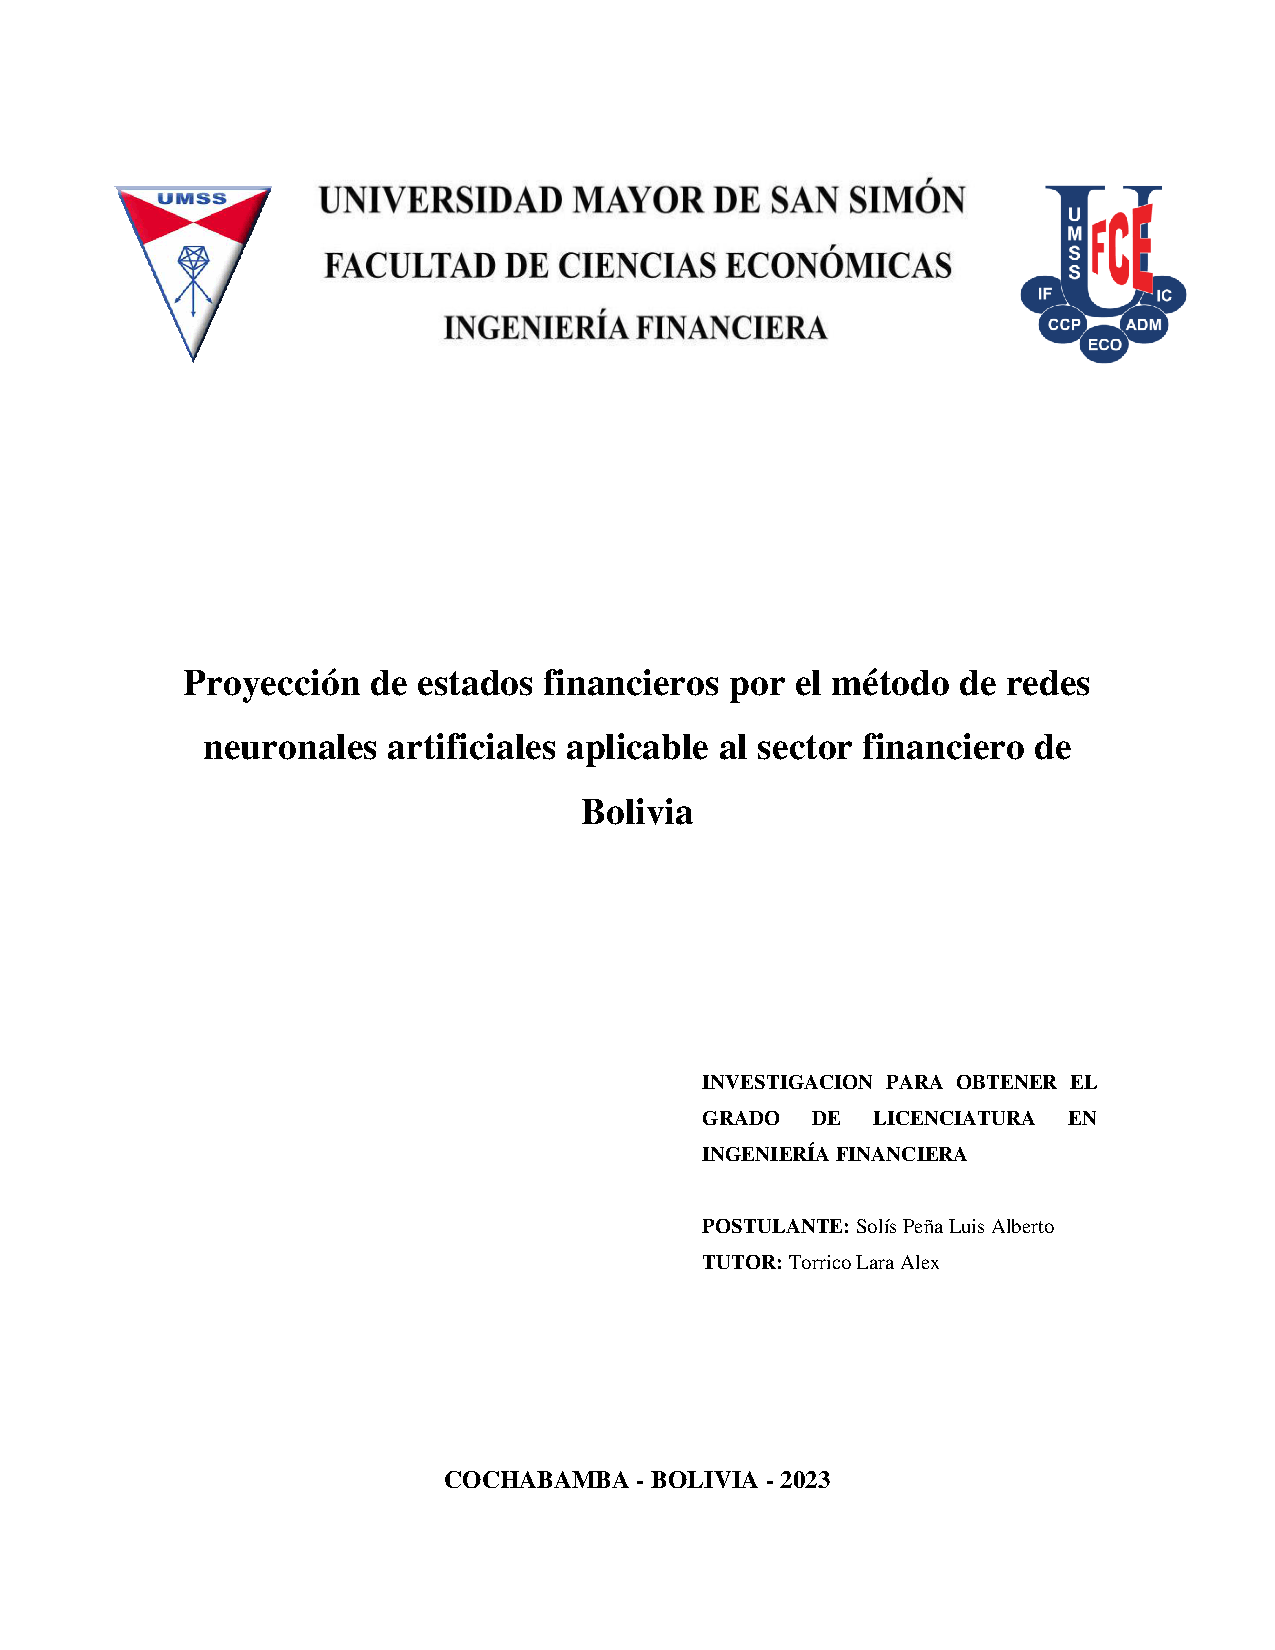
\includepdf[pages=-]{RECURSOS-INVESTIGACION/CARATULA-TESIS/CARATULA-TESIS}

\newpage
\tableofcontents
\listoffigures
\listoftables

\newpage

\hypertarget{perfil-de-la-investigaciuxf3n}{%
\section{Perfil de la
investigación}\label{perfil-de-la-investigaciuxf3n}}

\hypertarget{planteamiento-del-problema}{%
\subsection{Planteamiento del
problema}\label{planteamiento-del-problema}}

En un mundo cada vez más globalizado, y siendo el entorno financiero uno
de los sectores que más ha sido impactado por la integración económica
multilateral, que ha implicado su incremento en complejidad, donde los
agentes económicos son expuestos a una inmensa cantidad de información
sobre productos y/o servicios financieros, lo que puede dar lugar a
oportunidades de incrementar rendimientos, sin dejar de lado el riesgo
de perdidas consecuencia de la complejidad del mismo.

Una de las alternativas de tratamiento de esta información que ofrece el
sistema financiero, y que es el objeto de estudio en esta investigación
que se propone, es la aplicación de redes neuronales artificiales para
la proyección de estados financieros, la cual se encarga de encontrar la
relación existente en las variables introducidas al modelo que no pueden
ser visibles al análisis subjetivo económico-financiero, dando lugar a
la necesidad de evaluar dicha información por herramientas de igual
complejidad.

\begin{figure}[h!]
\centering
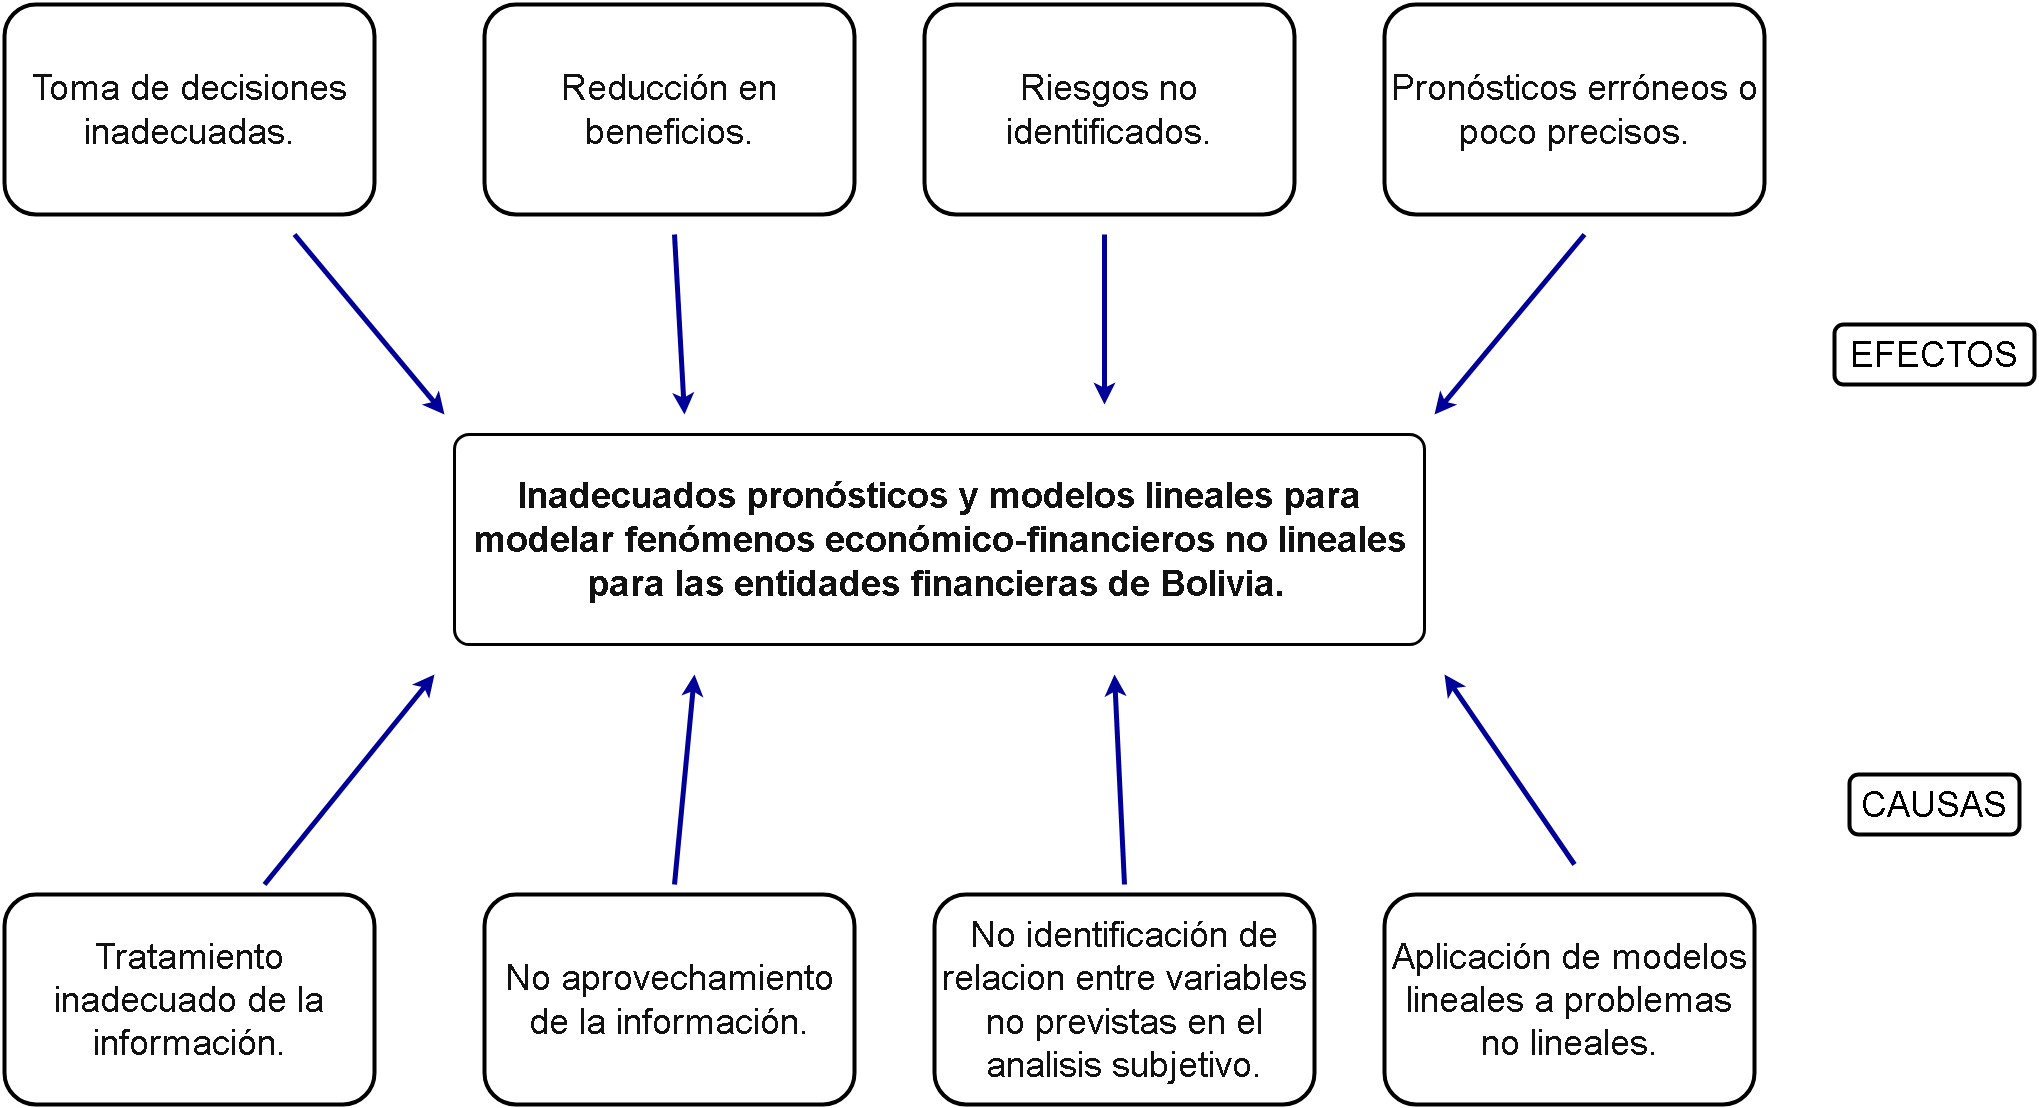
\includegraphics[width=15cm, height=10cm]{RECURSOS-INVESTIGACION/001-PERFIL-DEL-PROYECTO/arbol-de-problemas.png}
\caption{Arbol de problemas}
\end{figure}

\hypertarget{formulaciuxf3n-del-problema-central}{%
\subsection{Formulación del problema
central}\label{formulaciuxf3n-del-problema-central}}

¿Sera que con la aplicación del método de redes neuronales, se obtendrá
información adecuada con mayor aproximación a la situación
económica-financiera observada de la institución financiera
correspondiente?

\hypertarget{justificaciuxf3n}{%
\subsection{Justificación}\label{justificaciuxf3n}}

Observando la importancia de las proyecciones para la toma de
decisiones, y la capacidad de las redes neuronales de encontrar patrones
no visibles al análisis subjetivo, este tipo de modelos podrán dotar de
mayor información a agentes internos y externos del sector financiero de
donde y como hacer colocaciones o inversiones sobre el dinero que
administran.

En síntesis, el presente trabajo de investigación no pretende remplazar
a otros modelos existentes para la toma de decisiones, por el contrario,
ser tomado como una alternativa para el modelado de fenómenos no
lineales en el campo de las finanzas.

\hypertarget{alcance-y-delimitaciuxf3n}{%
\subsection{Alcance y delimitación}\label{alcance-y-delimitaciuxf3n}}

El presente trabajo de investigación se circunscribirá al estudio de las
entidades de intermediación de servicios financieras de Bolivia,
definidas en el artículo 151 de la ley 393. Con fines de obtener la
información que coadyuve a generar la determinación de pronósticos
mediante redes neuronales, como herramienta en la toma de decisiones a
nivel gerencial y la evaluación de las mismas.

Para viabilizar la realización del tema de investigación se ha elegido,
que se tomará como modelo de análisis a las siguientes entidades:

\begin{itemize}
\tightlist
\item
  Bancos múltiples.
\item
  Bancos PYME.
\item
  Entidades financieras de vivienda.
\item
  Cooperativas de ahorro y crédito abiertas.
\item
  Instituciones financieras de desarrollo.
\item
  Bancos de desarrollo productivo.
\end{itemize}

para tener acceso a la información homogénea requerida, que permita
generalizar los resultados mensuales obtenidos de las gestiones de 2014
a 2021, proyectando los periodos posteriores. El tema elegido y
propuesto, se realizará en un tiempo no mayor a diez meses, a partir de
la aprobación y registro del plan de investigación presentado.

\hypertarget{objetivos-de-la-investigaciuxf3n}{%
\subsection{Objetivos de la
investigación}\label{objetivos-de-la-investigaciuxf3n}}

Entre los objetivos propuestos para viabilizar el tema de investigación
y la realización del informe final, se describen los siguientes:

\hypertarget{general}{%
\subsubsection{General}\label{general}}

Proporcionar información financiera adecuada con mayor aproximación a la
situación económica-financiera observada, mediante la determinación de
pronósticos de estados financieros por el método de redes neuronales
artificiales.

\hypertarget{especifico}{%
\subsubsection{Especifico}\label{especifico}}

\begin{itemize}
\tightlist
\item
  Diagnostico de la situación actual del sistema financiero de Bolivia.
\item
  Definir la arquitectura y entrenamiento del modelo de red de neuronas
  artificiales.
\item
  Proyección y simulación de estados financieros.
\item
  Evaluación financiera sobre estados financieros proyectados-simulados.
\end{itemize}

\hypertarget{hipotesis}{%
\subsection{Hipotesis}\label{hipotesis}}

Con la determinación de proyecciones de estados financieros por el
método de redes neuronales, de entidades financieras de Bolivia, se
logrará proyectar información con mayor aproximación a la situación
económica-financiera observada de la institución correspondiente.

\hypertarget{elementos-o-componentes}{%
\subsubsection{Elementos o componentes}\label{elementos-o-componentes}}

\begin{itemize}
\tightlist
\item
  Unidad de observación y análisis: Entidades financieras de Bolivia.
\item
  Variable independiente: Proyecciones de estados financieros por el
  método de redes neuronales.
\item
  Variable dependiente: Información con mayor aproximación a la
  situación económica-financiera observada de la institución
  correspondiente.
\item
  Enlace lógico: Se logrará.
\end{itemize}

\hypertarget{marco-metoduxf3logico}{%
\subsection{Marco metodólogico}\label{marco-metoduxf3logico}}

\hypertarget{tipo-de-investigaciuxf3n}{%
\subsubsection{Tipo de investigación}\label{tipo-de-investigaciuxf3n}}

El tipo de investigación que se aplicará en el informe final será el
descriptivo y analítico, donde se busca describir y estudiar la realidad
presente de los hechos de las unidades de observación y análisis.

\hypertarget{muxe9todo-de-investigaciuxf3n}{%
\subsubsection{Método de
investigación}\label{muxe9todo-de-investigaciuxf3n}}

Donde se aplicará un enfoque inductivo donde desde hechos particulares
se llegará a conclusiones generales, que posteriormente puedan ser
aplicadas en otras instituciones financieras de manera exitosa y
beneficiar al sistema financiero con nuestra propuesta. También cabe
especificar que los procedimientos a ser aplicados en el informe final,
estarán orientados a los métodos inductivo, deductivo, analítico
fundamentalmente.

\hypertarget{tecnicas-de-investigaciuxf3n}{%
\subsubsection{Tecnicas de
investigación}\label{tecnicas-de-investigaciuxf3n}}

En primera instancia se realizara la identificación del problema de
investigación que ya esta establecida en el proyecto de grado, donde se
identificará la arquitectura de la red neuronal, que está compuesta de
las funciones de activación, y ajuste de los datos en formato de tablas.
Posteriormente se realizará la etapa de recolección de datos e
información del sistema financiero correspondiente a las fuentes
secundarias. Para que en consecuencia con la obtención de la información
se realizara el ordenamiento de dicha información recopilada para su
procesamiento que permitirá dar un análisis concreto y preciso y a la
vez realizar su sistematización para la obtención del diagnóstico.

\newpage
\begin{table}[h!]

\centering

\caption{Matriz de diseño metodológico.}
\label{tab:matriz-metodologico}

\resizebox{16cm}{!} {

\begin{tabular}{|c|cccc|}
\hline
\textbf{\begin{tabular}[c]{@{}c@{}}Pregunta de \\ investigación\end{tabular}} & \multicolumn{4}{c|}{\begin{tabular}[c]{@{}c@{}}¿Será que con la aplicación del método de redes neuronales, se obtendrá \\ información adecuada con mayor aproximación a la situación \\ económica-financiera de la institución financiera analizada?\end{tabular}} \\ \hline
\textbf{\begin{tabular}[c]{@{}c@{}}Objetivo \\ general\end{tabular}} & \multicolumn{4}{c|}{\begin{tabular}[c]{@{}c@{}}Proporcionar información financiera adecuada con mayor aproximación a la de \\ decisiones situación económica-financiera observada, mediante la determinación \\ de pronósticos de estados financieros por el método de redes neuronales artificiales.\end{tabular}} \\ \hline
\textbf{\begin{tabular}[c]{@{}c@{}}Objetivos \\ específicos\end{tabular}} & \multicolumn{1}{c|}{\begin{tabular}[c]{@{}c@{}}Diagnosticar la \\ situación actual \\ del sistema financiero \\ de Bolivia\end{tabular}} & \multicolumn{1}{c|}{\begin{tabular}[c]{@{}c@{}}Definir la \\ arquitectura y \\ entrenamiento \\ del modelo de red \\ de neuronas \\ artificiales\end{tabular}} & \multicolumn{1}{c|}{\begin{tabular}[c]{@{}c@{}}Proyectar \\ los estados \\ financieros \\ para su\\  posterior \\ simulación\end{tabular}} & \begin{tabular}[c]{@{}c@{}}Evaluar \\ los datos \\ proyectados-simulados \\ respecto a los datos \\ observados\end{tabular} \\ \hline
\textbf{\begin{tabular}[c]{@{}c@{}}Unidad de \\ análisis\end{tabular}} & \multicolumn{1}{c|}{CAMEL} & \multicolumn{1}{c|}{\begin{tabular}[c]{@{}c@{}}RED\\ NEURONAL\end{tabular}} & \multicolumn{1}{c|}{\begin{tabular}[c]{@{}c@{}}RED\\ NEURONAL\end{tabular}} & CAMEL \\ \hline
\textbf{\begin{tabular}[c]{@{}c@{}}Tipo de \\ fuente\end{tabular}} & \multicolumn{1}{c|}{Secundaria} & \multicolumn{1}{c|}{Secundaria} & \multicolumn{1}{c|}{Secundaria} & Secundaria \\ \hline
\textbf{\begin{tabular}[c]{@{}c@{}}Técnica de \\ recolección\end{tabular}} & \multicolumn{1}{c|}{\begin{tabular}[c]{@{}c@{}}Revisión \\ bibliográfica\end{tabular}} & \multicolumn{1}{c|}{\begin{tabular}[c]{@{}c@{}}Revisión \\ bibliográfica\end{tabular}} & \multicolumn{1}{c|}{\begin{tabular}[c]{@{}c@{}}Revisión \\ bibliográfica\end{tabular}} & \begin{tabular}[c]{@{}c@{}}Revisión \\ bibliográfica\end{tabular} \\ \hline
\textbf{\begin{tabular}[c]{@{}c@{}}Información \\ necesaria\end{tabular}} & \multicolumn{1}{c|}{\begin{tabular}[c]{@{}c@{}}Estados Financieros \\ del sistema financiero \\ de Bolivia.\end{tabular}} & \multicolumn{1}{c|}{\begin{tabular}[c]{@{}c@{}}Elementos de la \\ red neuronal, \\ número de neuronas, \\ funciones de activación \\ y funciones de coste.\end{tabular}} & \multicolumn{1}{c|}{\begin{tabular}[c]{@{}c@{}}Estados financieros \\ estructurados en \\ forma vectores.\end{tabular}} & \begin{tabular}[c]{@{}c@{}}Estados \\ financieros \\ proyectados.\end{tabular} \\ \hline
\end{tabular}

}
\floatfoot{Fuente: Elaboración propia.}
\end{table}


\hypertarget{fuentes-de-informaciuxf3n}{%
\subsection{Fuentes de información}\label{fuentes-de-informaciuxf3n}}

Se recurrirá a las fuentes de información siguientes:

\hypertarget{fuentes-primarias}{%
\subsubsection{Fuentes primarias}\label{fuentes-primarias}}

Se recurrirá a la investigación y recopilación de datos relacionados al
tema específico, mediante consultas a libros, revistas, textos
digitales, apuntes de clases y otras de información histórica.

\hypertarget{fuentes-secundarias}{%
\subsubsection{Fuentes secundarias}\label{fuentes-secundarias}}

Se recurrirá a las fuentes de compilación de información bibliográfica
referente al tema, tales como:

\begin{itemize}
\tightlist
\item
  libros especializados.
\item
  leyes.
\item
  normas.
\item
  resoluciones.
\item
  glosarios.
\item
  páginas de Internet.
\end{itemize}

\hypertarget{tuxe9cnica-de-recolecciuxf3n-de-la-informaciuxf3n}{%
\subsubsection{Técnica de recolección de la
información}\label{tuxe9cnica-de-recolecciuxf3n-de-la-informaciuxf3n}}

\begin{itemize}
\tightlist
\item
  Recopilación de información basada en fuentes primarias, secundarias y
  terciarias.
\item
  Análisis de la información recopilada, con fines de depuración,
  selección, tabulación mediante lenguajes de programación R y Python
  orientado al análisis de datos, adecuando a la arquitectura de la red
  neuronal.
\end{itemize}

\newpage

\hypertarget{antecedentes}{%
\section{Antecedentes}\label{antecedentes}}

Los antecedentes presentados a continuación cubren dos segmentos el
campo de las finanzas y el campo de las redes neuronales, considerando
también como convergen ambos en el tiempo.

La finanzas como ciencia es el resultado de la contribución de varios
individuos en diferentes puntos de tiempo y también como consecuencia de
otras ciencias sociales, siendo la ciencias contables y administrativas
las bases de la misma, las ciencias contable dotando la materia prima y
las administrativas los métodos, con este contexto presentamos los
antecedentes financieros generales:

En 1494 en Venecia el Fray Luca Pacioli en su obra ``Summa'' presento un
análisis sistemático del método contable dando lugar principio de doble
partida.

Pero solo en 2001, la ciencia contable llego a uno de sus primeras
cumbres que formalizan sus conocimientos con las normas internacionales
de contabilidad, de la mano del Comité de Normas Internacionales de
Contabilidad.

Ahora por el lado del redes neuronales artificiales se nombran los
siguientes antecedentes:

Como antecedentes generales, muestran que los inicios de la inteligencia
artificial de manera formal se dieron en el año 1943 cuando se colocó la
primera piedra angular sobre la que se basó lo que hoy se conoce como
inteligencia artificial, de la mano de Warren McCulloch y Walter Pitts,
con la presentación del primer modelo matemático de aprendizaje, donde
por primera vez se dota a un modelo autónomo la capacidad de
aprendizaje.

En 1949 se dio otro aporte al campo de las redes neuronales por parte de
Donald Hebb, quien fue el primero en explicar los procesos del
aprendizaje desde una perspectiva del campo psicológico, desarrollando
una regla de como el aprendizaje ocurría. La idea general que propuso
era que el aprendizaje ocurría cuando ciertos cambios en una neurona
eran activados.

En 1950 Alam Turing presento lo que se denominó como la ``Prueba de
Turing'', donde dio una definición operacional y satisfactoria de
inteligencia, que dicha prueba consistía en la incapacidad de
diferenciar entre entidades inteligentes indiscutibles y seres humanos.

Pero solo en 1957, Frank Rosenblatt pudo generalizar las ideas propuesta
por Warren McCulloch y Walter Pitts, a dicho modelo lo denomino
PERCEPTRON, el cual tiene la capacidad de generalizar problemas lineales
por medio de datos de ejemplo, donde reconoce patrones y hace
predicciones con datos diferentes con los que había sido entrenado, es
decir está dotado con la capacidad de generalizar, y 1959 Frank
Rosenblatt en su libro ``Principios de Neuro dinámica'' confirmó que,
bajo ciertas condiciones, el aprendizaje del Perceptrón convergía hacia
un estado finito que denomino teorema de convergencia del Perceptrón.

En 1960 Bernard Widroff y Marcian Hoff, desarrollaron el modelo ADELINE
(ADAptative LINear Elements) que fue la primera aplicación comercial de
redes neuronales para eliminar ecos en las líneas telefónicas. En 1969
se produjo un declive en las redes neuronales en consecuencia, de una
publicación de Marvin Minsky y Seymour Papert probaron matemáticamente
que, si bien el perceptrón era capaz de resolver con facilidad problemas
lineales, pero su rendimiento decaía cuando intentaba modelar problemas
no lineales, sobrecargando la capacidad computo.

Pero en 1985 John Hopfield, hizo que las redes neuronales cobraran
nuevamente importancia con su libro ``Computación neuronal de decisiones
en problemas de optimización'' donde presenta el algoritmo de
retropropagación que reduce cantidad de cómputo en proceso de
aprendizaje de las redes neuronales, dotando a esta de la capacidad de
resolver problemas no lineales. También 1986 David E. Rumelhart y
Geoffrey E. Hinton, mejoraron el algoritmo de aprendizaje de propagación
hacia atrás, que permitieron recortar el tiempo aún más el proceso de
aprendizaje con respecto a los modelos anteriores.

Uno de los aportes más recientes vino por parte de la Universidad de
Toronto y la empresa de Google en 2017 con la publicación del articulo
titulado ``Atención es todo lo que necesitas'', con la presentación de
la arquitectura denominada ``transformes'' que de la mano de las redes
neuronales dotan de atención al modelo de inteligencia artificial.

Ahora bien como antecedentes específicos Bolivia no es un país que lleve
adelante de investigación o desarrollos significativos sobre
inteligencia artificial como un dato relevante según el reporte
Government AI Readiness Index 2020 (Oxford Insights), Bolivia ocupa el
puesto 122 de 172 países, y el 22 de 32 en la región de Latinoamérica y
el Caribe.

Concluyendo la sección el punto temporal la que se hace manifiesto que
convergen el campo de las ciencias sociales y los modelos
matemáticos-estadísticos fue traído de la mano de Francis Galton en
1886, quien acuño el términos de regresión en su articulo ``Semejanza
familiar en estatura'', la hipótesis propuesta en este articulo fue
contrastada por Karl Pearson dando lugar a la ley de regresión
universal, desde este punto hasta la actualidad los métodos de regresión
han evolucionado llegando a los métodos mas actuales y complejos como
son las redes neuronales artificiales.

\newpage

\hypertarget{marco-teorico}{%
\section{Marco teorico}\label{marco-teorico}}

\hypertarget{finanzas-y-el-sistema-financiero}{%
\subsection{Finanzas y el sistema
financiero}\label{finanzas-y-el-sistema-financiero}}

Las finanzas se entiende como ``la ciencia y arte de administrar el
dinero'' sujetas a restricciones dadas por un contexto que es dado por
el sistema financiero, en decir, el sistema financiero, ``consiste en
diversas instituciones y mercados que sirven a las empresas de negocios,
los individuos y los gobiernos''.(James C. Van Horne, 2010)

Entonces se afirma que el sistema financiero en general está formado por
el conjunto de instituciones publicas y privadas, constituidas en
mercados, cuyo fin principal es canalizar el ahorro que generan los
ahorradores hacia los prestatarios, así como facilitar y otorgar
seguridad al movimiento de dinero y al sistema de pagos.

\hypertarget{entidades-de-intermediaciuxf3n-financiera-en-bolivia}{%
\subsubsection{Entidades de intermediación financiera en
Bolivia}\label{entidades-de-intermediaciuxf3n-financiera-en-bolivia}}

Las definiciones presentadas a continuación están suscritas a la ley 393
- ley de servicios financieros.

\hypertarget{bancos-muxfaltiples.}{%
\paragraph{Bancos múltiples.}\label{bancos-muxfaltiples.}}

Los bancos múltiples tendrán como objetivo la prestación de servicios
financieros al publico en general, entendido como servicios financieros,
aquellos servicios que tienen por objeto satisfacer las necesidades de
las consumidoras y consumidores financieros.

\hypertarget{bancos-pyme}{%
\paragraph{Bancos PYME}\label{bancos-pyme}}

Los bancos PYME son aquellos que tienen como objetivo la prestación de
servicios financieros especializados en el sector de las pequeñas y
medianas empresas, sin restricción para la prestación de los mismos
también a la microempresa.

\hypertarget{entidades-financieras-de-vivienda}{%
\paragraph{Entidades financieras de
vivienda}\label{entidades-financieras-de-vivienda}}

Las entidades financieras de vivienda es una sociedad que tiene por
objeto prestar servicios de intermediación financiera con
especialización en prestamos para adquisición de vivienda, proyectos de
construcción de vivienda unifamiliar o multifamiliar, compra de
terrenos, refacción, remodelación, ampliación y mejoramiento de
viviendas individuales o propiedad horizontal y otorgamiento de
microcredito para vivienda familiar y para infraestructura de vivienda
productiva, así tambien operaciones de arrendamiento financiero
habitacional.

\hypertarget{cooperativas-de-ahorro-y-cruxe9dito-abiertas}{%
\paragraph{Cooperativas de ahorro y crédito
abiertas}\label{cooperativas-de-ahorro-y-cruxe9dito-abiertas}}

Las cooperativas de ahorro y crédito se constituyen como entidades
especializadas de objeto único para la prestación de servicios de
intermediación financiera, dirigidos a sus socios y al publico en
general cunado corresponda.

\hypertarget{instituciones-financieras-de-desarrollo}{%
\paragraph{Instituciones financieras de
desarrollo}\label{instituciones-financieras-de-desarrollo}}

La institución financiera de desarrollo es una organización jurídica
propia creada con el objeto de prestar servicios financieros con un
enfoque integral que incluye gestión social.

\hypertarget{bancos-de-desarrollo-productivo}{%
\paragraph{Bancos de desarrollo
productivo}\label{bancos-de-desarrollo-productivo}}

El banco de desarrollo productivo es una institución con participación
mayoritaria del estado que realiza actividades de primer y segundo piso
de fomento y de promoción del desarrollo del sector productivo.

\hypertarget{estados-financieros}{%
\subsection{Estados financieros}\label{estados-financieros}}

En el campo de la ciencia económicas los estados financieros tiene como
objeto reflejar la situación económica-financiera de una institución.

En la página oficial de la Autoridad de Supervisión del Sistema
Financiero (ASFI), ``se define que los estados financieros constituyen
una representación estructurada de la situación financiera y de las
transacciones llevadas a cabo por la empresa. Su objetivo, con
propósitos de información general, es suministrar información acerca de
la situación y rendimiento financieros, así como de los flujos de
efectivo que sea útil a una amplia variedad de usuarios al tomar sus
decisiones económicas. Los estados financieros también muestran los
resultados de la gestión que los administradores han efectuado con los
recursos que se les han confiado''. (ASFI, 2022)

Entonces se afirma, que los estados financieros son un resumen del
ejercicio económico de una empresa o institución, entendiendo al
ejercicio económico como la suma de todas las actividades vinculadas al
giro de la empresa en un intervalo de tiempo, dando información, sobre
ingresos, egresos, pasivos, activos, es decir, los estados financieros
son una fotografía de la empresa en un punto del tiempo.

\hypertarget{balance-general}{%
\subsubsection{Balance general}\label{balance-general}}

El balance general se entiende como, ``estado financiero que muestra, a
una fecha determinada, el valor y la estructura del activo, pasivo y
patrimonio de una empresa''. (ASFI, 2022)

Con una expresión equivalente se afirma que el balance general
representa una fotografía sobre el estado de de los bienes y derechos,
respecto a las obligaciones con propietarios e terceros de la
institución en un determinado momento.

\hypertarget{estado-de-resultados}{%
\subsubsection{Estado de resultados}\label{estado-de-resultados}}

Estado de ganancias y pérdidas o estado de resultados, se entiende como,
``documento contable que muestra el resultado de las operaciones
(utilidad o pérdida) de una entidad durante un periodo y a una fecha
determinada; resulta de la comparación de los ingresos con los gastos
efectuados''. (ASFI, 2022)

Es decir, el estado de resultados muestra la conclusión en términos
monetarios del conjunto de actividades administrativas y complementarias
en un intervalo de tiempo de la institución correspondiente.

\hypertarget{evaluaciuxf3n-financiera}{%
\subsection{Evaluación financiera}\label{evaluaciuxf3n-financiera}}

La evaluación financiera se entiende como un proceso de valoración de
los resultados de actividades económica-financieras de las
instituciones.

\hypertarget{indicadores-financieros}{%
\subsubsection{Indicadores financieros}\label{indicadores-financieros}}

La teoría financiera indica que un indicador financiero tiene como
objeto final medir una característica de la entidad estudiada, estos
pueden ser los siguientes:

\begin{itemize}
\tightlist
\item
  Estructura de activos.
\item
  Estructura de pasivos.
\item
  Estructura de obligaciones.
\item
  Calidad de cartera.
\item
  Liquidez.
\item
  Rentabilidad.
\item
  Ingresos y gastos financieros.
\item
  Eficacia administrativas.
\end{itemize}

Pero los indicadores financieros por si solos no pueden brindar
información integrada sobre la situación económica-financiera de una
institución en consecuencia a esta necesidad, se encuentra las
metodologías de evaluación como ser la metodología CAMEL y PERLAS.

\hypertarget{muxe9todo-camel}{%
\subsection{Método CAMEL}\label{muxe9todo-camel}}

La metodología CAMEL evalúa la \textbf{solidez financiera} de las
instituciones con base ha indicadores cuantitativos, contemplando cinco
características:

\begin{itemize}
\tightlist
\item
  Capital adecuado (C).
\item
  Calidad del activo (A).
\item
  Capacidad de la gerencia (M).
\item
  Rentabilidad (E).
\item
  Situación de liquidez (L).
\end{itemize}

La \textbf{solidez financiera} de una institución debe entenderse como
la capacidad que tiene dicha institución de hacer frente a las
obligaciones que tiene con terceros y propietarios.

La presente metodología se divide en siguientes pasos:

\begin{itemize}
\tightlist
\item
  Calculo de indicadores que responden a los características antes
  mencionadas.
\item
  Definición de rangos y limites de los indicadores.
\item
  Definición de la ponderación, que responden a la solidez financiera de
  la institución.
\item
  Calificación CAMEL.
\end{itemize}

Los mismos que se describen a continuación:

\hypertarget{calculo-de-indicadores}{%
\subsubsection{Calculo de indicadores}\label{calculo-de-indicadores}}

\hypertarget{capital}{%
\paragraph{Capital}\label{capital}}

\hypertarget{coeficiente-de-adecuaciuxf3n-patrimonial}{%
\subparagraph{Coeficiente De Adecuación
Patrimonial}\label{coeficiente-de-adecuaciuxf3n-patrimonial}}

Está definido cómo la relación porcentual entre el capital regulatorio y
los activos y contingentes ponderados en función de factores de riesgo,
incluyendo a los riesgos de crédito, de mercado y operativo, utilizando
los procedimientos establecidos en la normativa emitida por la Autoridad
de Supervisión del Sistema Financiero - ASFI.

\hypertarget{coeficiente-de-covertura-de-cartera-en-mora}{%
\subparagraph{Coeficiente De Covertura De Cartera En
Mora}\label{coeficiente-de-covertura-de-cartera-en-mora}}

Este indicador mide o tiene objeto responder si el patrimonio de la
institución cubre en tanto por ciento: - Los créditos cuyo capital,
cuotas de amortización o intereses no hayan sido cancelados íntegramente
a la entidad hasta los 30 días contados desde la fecha de vencimiento. -
Los créditos por los cuales la entidad ha iniciado las acciones
judiciales para el cobro. - Descontando la previsión por incobrabilidad
de créditos.

\[ \frac{ \text{Cartera En Mora - Previsión Cartera} }{\text{Patrimonio}}\]

\hypertarget{coeficiente-acido-de-covertura-de-cartera-en-mora}{%
\subparagraph{Coeficiente Acido De Covertura De Cartera En
Mora}\label{coeficiente-acido-de-covertura-de-cartera-en-mora}}

Este indicador mide o tiene objeto responder si el patrimonio de la
institución cubre en tanto por ciento: - Los créditos cuyo capital,
cuotas de amortización o intereses no hayan sido cancelados íntegramente
a la entidad hasta los 30 días contados desde la fecha de vencimiento. -
Los créditos por los cuales la entidad ha iniciado las acciones
judiciales para el cobro. - Descontando la previsión por incobrabilidad
de créditos y adjuntando bienes realizables.

\[ \frac{ \text{Cartera De Mora - Previsión Carter + Realizables} }{ \text{Patrimonio} } \]

\hypertarget{coeficiente-de-cobertura-patrimonial}{%
\subparagraph{Coeficiente de cobertura
patrimonial}\label{coeficiente-de-cobertura-patrimonial}}

Este indicador mide o tiene por objeto responder si los activos
descontando los cuentas contingentes cubren los el patrimonio de la
misma.

\[ \frac{ \text{Patrimonio} }{ \text{Activo - Contingente} } \]

\hypertarget{activo}{%
\paragraph{Activo}\label{activo}}

\hypertarget{coeficiente-de-exposiciuxf3n-de-cartera}{%
\subparagraph{Coeficiente de exposición de
cartera}\label{coeficiente-de-exposiciuxf3n-de-cartera}}

El presente coeficiente determina que por ciento de lo créditos están
expuestos a riesgo de ser incumplidos o cancelados.

\[  \frac{ \text{Cartera En Mora} }{ \text{Cartera Bruta} } \]

\hypertarget{coeficiente-de-previsiuxf3n-de-cartera}{%
\subparagraph{Coeficiente de previsión de
cartera}\label{coeficiente-de-previsiuxf3n-de-cartera}}

El presente coeficiente mide o tiene por objeto responder en que tanto
por ciento esta cubierta los créditos realizados por la institución.

\[ \frac{ \text{Prevision} }{ \text{Cartera Bruta} } \]

\hypertarget{coeficiente-de-previsiuxf3n-de-cartera-en-mora}{%
\subparagraph{Coeficiente de previsión de cartera en
mora}\label{coeficiente-de-previsiuxf3n-de-cartera-en-mora}}

Este coeficiente mide o tiene por objeto responder en que tanto por
ciento esta cubierta los créditos incobrables realizados por la
institución.

\[ \frac{ \text{Prevision} }{ \text{Cartera En Mora} } \]

\hypertarget{coeficiente-de-reposiciuxf3n-de-cartera}{%
\subparagraph{Coeficiente de reposición de
cartera}\label{coeficiente-de-reposiciuxf3n-de-cartera}}

Dicho coeficiente tiene por objeto medir en que tanto por ciento
alcanzan los créditos re programados.

\[ \frac{ \text{Cartera Reprogramada Total} }{ \text{Cartera Bruta} } \]

\hypertarget{administraciuxf3n}{%
\paragraph{Administración}\label{administraciuxf3n}}

\hypertarget{coeficiente-de-cobertura-gastos-administrativos}{%
\subparagraph{Coeficiente de cobertura gastos
administrativos}\label{coeficiente-de-cobertura-gastos-administrativos}}

El coeficiente mide si los activos de la institución pueden hacer frente
a los gastos administrativos de la institución.

\[ \frac{ \text{Gastos Administración} }{ \text{Activos + Contingentes} } \]

\hypertarget{coeficiente-acido-de-cobertura-patrimonial}{%
\subparagraph{Coeficiente acido de cobertura
patrimonial}\label{coeficiente-acido-de-cobertura-patrimonial}}

Este coeficiente mide si los ingresos brutos pueden hacer frente a los
gastos administrativos de la institución.

\[ \frac{ \text{Gastos Administración - Impuestos} }{ \text{Resultado Operativo Bruto} } \]

\hypertarget{beneficios}{%
\paragraph{Beneficios}\label{beneficios}}

\hypertarget{coeficiente-de-rendimiento-sobre-activos}{%
\subparagraph{Coeficiente de rendimiento sobre
activos}\label{coeficiente-de-rendimiento-sobre-activos}}

El presente coeficiente determina el rendimiento en tanto por uno, los
beneficios que han generado los activos.

\[ \frac{ \text{Resultado Neto De La Gestión} }{ \text{Activo+Contingente} } \]

\hypertarget{coeficiente-de-rendimiento-sobre-patrimonio}{%
\subparagraph{Coeficiente de rendimiento sobre
patrimonio}\label{coeficiente-de-rendimiento-sobre-patrimonio}}

Este coeficiente determina el rendimiento en tanto por uno, los
beneficios que ha generado el patrimonio.

\[ \frac{ \text{Resultado Neto De La Gestión} }{ \text{Patrimonio} } \]

\hypertarget{liquidez}{%
\paragraph{Liquidez}\label{liquidez}}

\hypertarget{coeficiente-de-capacidad-de-pago-frente-obligaciones-a-corto-plazo}{%
\subparagraph{Coeficiente de capacidad de pago frente obligaciones a
corto
plazo}\label{coeficiente-de-capacidad-de-pago-frente-obligaciones-a-corto-plazo}}

El coeficiente busca medir si la institución puede hacer frente a sus
obligaciones con los activos disponibles y inversiones temporales.

\[ \frac{ \text{Disponibles + Inversiones Temporarias} }{ \text{Obligaciones A Corto Plazo} } \]

\hypertarget{coeficiente-acido-de-capacidad-de-pago-frente-obligaciones-a-corto-plazo}{%
\subparagraph{Coeficiente acido de capacidad de pago frente obligaciones
a corto
plazo}\label{coeficiente-acido-de-capacidad-de-pago-frente-obligaciones-a-corto-plazo}}

El coeficiente busca medir si la institución puede hacer frente a sus
obligaciones con los activos disponibles.

\[ \frac{ \text{Disponibles} }{ \text{Obligaciones A Corto Plazo} } \]

\hypertarget{definiciuxf3n-de-rangos-y-limites-de-los-indicadores}{%
\subsubsection{Definición de rangos y limites de los
indicadores}\label{definiciuxf3n-de-rangos-y-limites-de-los-indicadores}}

En esta sección de la metodología CAMEL se establecen rangos a los
cuales le corresponde una calificación, sujeta a una probabilidad, es
decir, aquellos resultados mejores pero menos probable reciben una mejor
calificación y aquellos resultados peores y menos probables reciben una
peor calificación.

\begin{table}[h!]

\centering
\caption{Calificación CAMEL}
\label{tab:calificacion-camel-marco-teorico}

\begin{tabular}{|c|c|c|}
\hline
\textbf{Raiting} & \textbf{Descripción} & \textbf{Significado}            \\ \hline
1                & Robusto              & Solvente en todos aspectos      \\ \hline
2                & Satisfactorio        & Generalmente solvente           \\ \hline
3                & Normal               & Cierto nivel de vulnerabilidad  \\ \hline
4                & Marginal             & Problemas financieros serios    \\ \hline
5                & Insatisfactorio      & Serios problemas de solidez \\ \hline

\multicolumn{3}{c}{\footnotesize Nota: Obtenido de (Alpiry Hurtado, 2021a).}

\end{tabular}

 
\end{table}




\hypertarget{definiciuxf3n-de-la-ponderaciuxf3n}{%
\subsubsection{Definición de la
ponderación}\label{definiciuxf3n-de-la-ponderaciuxf3n}}

\[CAMEL = \text{30\%C + 20\%A + 10\%M + 15\%E + 15\%L}\]

\hypertarget{calificaciuxf3n-camel}{%
\subsubsection{Calificación CAMEL}\label{calificaciuxf3n-camel}}

Dado los pasos anteriores la metodología CAMEL asigna una puntuación a
la institución, y permitirá determinar que institución le corresponde
mayor solidez financiera respecto a las otras instituciones.

\hypertarget{pronuxf3sticos}{%
\subsection{Pronósticos}\label{pronuxf3sticos}}

El termino de pronóstico de uso común, definido por la Real Academia
Española (RAE) como la acción y efecto de pronosticar, la misma RAE
define pronosticar como predecir algo en el futuro a partir de indicios.
El pronóstico es el proceso de estimación en situaciones de
incertidumbre, para los propósitos de esta investigación, un pronóstico
es un evento asociado a una distribución de probabilidad.

En consecuencia los pronósticos por si solos tampoco pueden brindar
información integrada sobre la situación económica-financiera futura de
la institución, en consecuencia a esta necesidad, se encuentra las
metodologías de evaluación junto con la simulación de procesos
estocásticos.

\hypertarget{inteligencia-artificial}{%
\subsection{Inteligencia artificial}\label{inteligencia-artificial}}

``En la literatura referente a la inteligencia artificial no existe
consenso sobre lo que se entiende como inteligencia artificial, pero
estas diferencias se engloban en dos ideas, donde la inteligencia
artificial se refieren a procesos mentales y al razonamiento''.(Stuart
Russell, 2004)

Ahora bien el campo de la inteligencia artificial es relativamente
reciente, y cobra atención en la actualidad por su capacidad de resolver
problemas que con anterioridad sus resultados se divisaban lejanos, como
el pronóstico de fenómenos no lineales, procesamientos de lenguaje
natural, generador de imágenes, clasificación de objetos e procesos
estocásticos donde se encuentra la proyección de estados financieros.

\hypertarget{aprendizaje-supervisado-con-redes-neuronales}{%
\subsubsection{Aprendizaje supervisado con redes
neuronales}\label{aprendizaje-supervisado-con-redes-neuronales}}

El aprendizaje supervisado corresponde a la situación en que se tiene
una variable de salida, ya sea cuantitativa o cualitativa, que se desea
predecir basándose en un conjunto de características.(Julio Cesar Ponce
Gallegos, 2014)

\textbf{El aprendizaje supervisado es una rama del aprendizaje
automático, son algoritmos que permiten aprender a la red neuronal
mediante datos ejemplos que están compuesta por un vector de entrada que
son las variables independientes, y otro vector denomina etiquetas,
donde la red se encarga de encontrar las relaciones existentes entre las
variables independientes, realizando cambios y adaptando el modelo por
medio de variaciones sujetas a una función de coste.}

\hypertarget{aprendizaje-no-supervisado-con-redes-neuronales}{%
\subsubsection{Aprendizaje no supervisado con redes
neuronales}\label{aprendizaje-no-supervisado-con-redes-neuronales}}

El aprendizaje no supervisado, ``corresponde a la situación en que
existe un conjunto de datos que contienen diversas características de
determinados individuos, sin que ninguna de ellas se considere una
variable de salida que se desee predecir''.(Julio Cesar Ponce Gallegos,
2014)

Aprendizaje no supervisado es un método de aprendizaje automático donde
la red neuronal se ajusta a las observaciones. Se distingue del
aprendizaje supervisado por el hecho de que no hay un conocimiento a
priori es decir etiquetas que sirvan como guía, en el aprendizaje no
supervisado solo se cuenta con un conjunto de datos de objetos de
entrada.

\hypertarget{redes-neuronales-artificiales}{%
\subsection{Redes neuronales
artificiales}\label{redes-neuronales-artificiales}}

Las Redes Neuronales ``son un paradigma de aprendizaje y procesamiento
automático inspirado en la forma en que funciona el cerebro para
realizar las tareas de pensar y tomar decisiones (sistema
nervioso)''.(Julio Cesar Ponce Gallegos, 2014)

Una red neuronal es un método del aprendizaje automático que enseña a
las computadoras a procesar datos de una manera que está inspirada en la
forma en que lo hace el cerebro humano, las redes neuronales
artificiales es modelo computacional resultado de diversas aportaciones
científicas, consiste en un conjunto de unidades llamadas neuronas
artificiales.

\hypertarget{elementos-de-redes-neuronales}{%
\subsection{Elementos de redes
neuronales}\label{elementos-de-redes-neuronales}}

Como todo sistema es el resultado de la interacción de elementos simples
trabajando conjuntamente, que se presenta a continuación.

\hypertarget{neurona-artificial}{%
\subsubsection{Neurona artificial}\label{neurona-artificial}}

La neurona es la unidad básica de procesamiento de una red neuronal de
ahí el nombre, igual que su equivalente biológico una neurona artificial
recibe estímulos externos y devuelve otro valor, esta es expresada
matemáticamente como una función, donde la neurona realiza una suma
ponderada con los datos de entrada.

Dado:

\[ X = \left( x_{1},x_{2},x_{3},...,x_{n} \right) \] Se tiene:
\[ Y = f(X) = \sum_{i=1}^{n}{w_{i}x_{i}}  = \sum{WX}  \] Donde: \newline
X = Vector de los datos de entrada. \newline Y = Vector resultado de la
suma ponderada. \newline W = Vector de los pesos las variables
independientes.

La arquitectura de la red neuronal corresponde a la manera en que esta
ordena las neuronas, si las neuronas son colocadas de forma vertical,
reciben los mismos datos de entrada y sus resultados de salida lo pasan
a la siguiente capa, la última capa de una red neuronal se denominan
capa de salida y las capas que estén entre la capa de salida y capa de
entrada se denominas capas ocultas. Ahora bien, al ser cada neurona una
suma ponderada esta equivaldría a una sola capa de la red, a esto se
denomina colisión de la red neuronal, para resolver este problema se
planteó los que se conoce como función de activación que es una función
no lineal que distorsiona los resultados salientes de cada neurona.

\[A = f(Y)\]

Dado lo anterior expuesto una capa de una red neuronal se debe entender
como la agrupación neuronas.

\hypertarget{funciones-de-activaciuxf3n}{%
\subsubsection{Funciones de
activación}\label{funciones-de-activaciuxf3n}}

Las funciones de activación distorsionan de forma no lineal las salidas
de las neuronas para así no colapsar la red, es decir, las funciones de
activación permiten conectar capas neuronales, dentro las funciones de
activación más conocidas se tiene:

\hypertarget{funciuxf3n-escalon}{%
\paragraph{Función escalon}\label{funciuxf3n-escalon}}

Esta función asigna el valor de 1 si la salida de la neurona supera
cierto umbral y cero si no lo supera.

\[ f(x) = max(0,x) = \left \{
\begin{array}{rcl}
     0 & Si & x < 0
  \\ 1 & Si & x \geq{0}
\end{array}
\right. \]

\hypertarget{funciuxf3n-sigmoide}{%
\paragraph{Función sigmoide}\label{funciuxf3n-sigmoide}}

Esta función genera un en un rango de valores de salida que están entre
cero y uno por lo que la salida es interpretada como una probabilidad.

\[ f(x) = \frac{1}{1+e^{-x}}\]

\hypertarget{funciuxf3n-tangente-hiperbuxf3lica}{%
\paragraph{Función tangente
hiperbólica}\label{funciuxf3n-tangente-hiperbuxf3lica}}

Esta función de activación llamada tangente hiperbólica tiene un rango
de valores de salida entre -1 y 1.

\[ f(x) = \frac{2}{1+e^{-2x}} - 1 \]

\hypertarget{funciuxf3n-relu}{%
\paragraph{Función Relu}\label{funciuxf3n-relu}}

La función ReLU transforma los valores introducidos anulando los valores
negativos y dejando los positivos.

\[ f(x) = max(0,x) = \left \{
\begin{array}{rcl}
     0 & Si & x < 0
  \\ x & Si & x \geq{0}
\end{array}
\right. \]

\hypertarget{funciuxf3n-leaky-relu}{%
\paragraph{Función Leaky ReLU}\label{funciuxf3n-leaky-relu}}

La función Leaky ReLU transforma los valores introducidos multiplicando
los negativos por un coeficiente rectificativo y dejando los positivos
según entran.

\[ f(x) = max(0,x) = \left \{
\begin{array}{rcl}
     0 & Si & x < 0
  \\ a*x & Si & x \geq{0}
\end{array}
\right. \]

\hypertarget{funciuxf3n-softmax}{%
\paragraph{Función Softmax}\label{funciuxf3n-softmax}}

La función Softmax transforma las salidas a una representación en forma
de probabilidades, de tal manera que el sumatorio de todas las
probabilidades de las salidas de 1.

\[ f(Z)_{j} = \frac{ e^{Z_{J}} }{ \sum_{k=1}^{K} e^{Z_{K}} } \]

\begin{figure}

{\centering 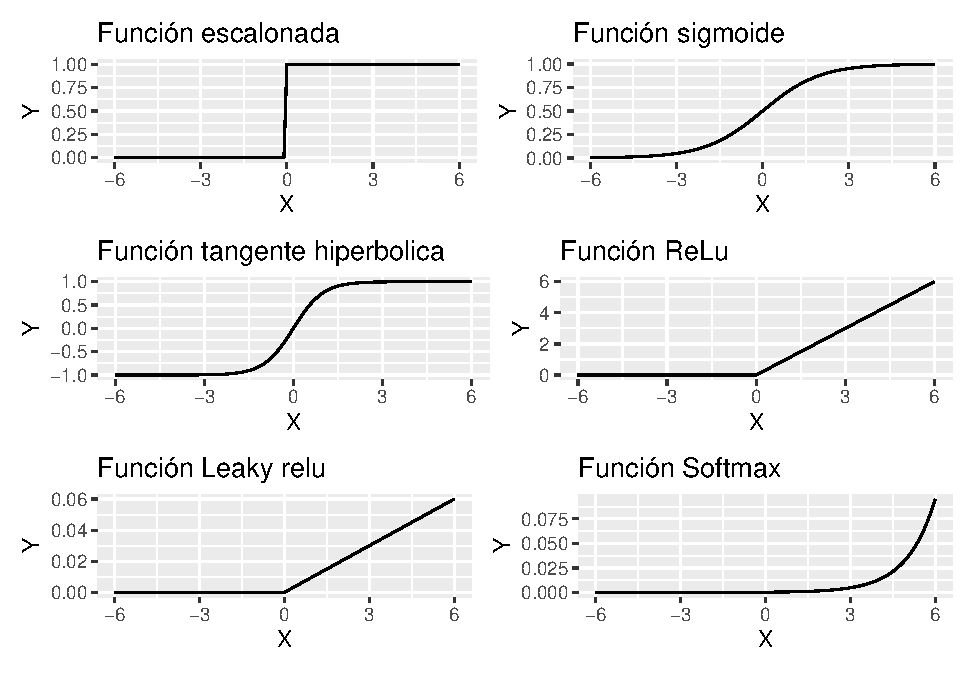
\includegraphics[width=1\linewidth,height=0.7\textheight]{PRINCIPAL-INVESTIGACION_files/figure-latex/unnamed-chunk-11-1} 

}

\caption{Funciones de activación}\label{fig:unnamed-chunk-11}
\end{figure}

\newpage

\hypertarget{propagaciuxf3n-hacia-adelanate-y-hacia-atras}{%
\subsubsection{Propagación hacia adelanate y hacia
atras}\label{propagaciuxf3n-hacia-adelanate-y-hacia-atras}}

\hypertarget{propagaciuxf3n-hacia-adelante}{%
\paragraph{Propagación hacia
adelante}\label{propagaciuxf3n-hacia-adelante}}

Para hacer manifiesto el algoritmo de propagación hacia adelante se
supone que la estructura de red, estará compuesta de de cuatro capas, es
decir, la capa de entrada y salida junto a dos capas neuronales ocultas,
dada esta estructura el algoritmo tendrá el siguiente comportamiento:

\begin{itemize}
\tightlist
\item
  Capa de entrada esta definida por:
\end{itemize}

\[ x = a^{(1)}\]

\begin{itemize}
\tightlist
\item
  La primera capa oculta procesara los datos de la capa de entrada toma
  la siguiente forma:
\end{itemize}

\[ z^{(2)} = W^{(1)}x + b^{(1)} \]

\begin{itemize}
\tightlist
\item
  Antes de pasar los datos procesados en las neuronas de la primera capa
  oculta deben ser pasados por las funcioes de activación, para que no
  colapse la red:
\end{itemize}

\[a^{(2)} = f(z^{(2)})\]

\begin{itemize}
\tightlist
\item
  Nuevamente se procesara los datos de la capa de anterior:
\end{itemize}

\[ z^{(3)} = W^{(2)}a^{(2)} + b^{(2)} \]

\begin{itemize}
\tightlist
\item
  Tambien nuevamente se envuelve los resultados en una función de
  activación antes de pasar a la capa de salida:
\end{itemize}

\[a^{(3)} = f(z^{(3)})\]

\begin{itemize}
\tightlist
\item
  Finalmente tendremos una salida, la cual sera evaluada si coincide con
  los datos esperados.
\end{itemize}

\[ s = W^{(3)}a^{(3)} \]

\hypertarget{propagaciuxf3n-hacia-atruxe1s}{%
\paragraph{Propagación hacia
atrás}\label{propagaciuxf3n-hacia-atruxe1s}}

El algoritmo de propagación hacia atrás o ``backpropagation'' tiene como
objeto dotar de aprendizaje a las redes neuronales minimizando la
función de costo ajustando los pesos y sesgos de la red, el nivel de
ajuste está determinado por los gradientes para cada neurona hasta
llegar a la capa de entrada.

Dada un función de costo:

\[ C = f(s,y) \]

Se calcula las derivadas parciales para cada neurona, para determinar
que rutas que han generado menor error, hasta la capa de entrada:

\[ \frac{ \partial{C} }{ \partial{x} }\]

Para el logro de esta derivada se hace uso de un método matemático
denominado ``Chain Rule'', que permite determinar la derivada de una
función compuesta, a través de funciones parciales de las funciones que
componen la función principal.

\newpage

\hypertarget{diagnuxf3stico-de-las-instituciones-financieras-del-sistema-financiero-de-bolivia}{%
\section{Diagnóstico de las instituciones financieras del sistema
financiero de
Bolivia}\label{diagnuxf3stico-de-las-instituciones-financieras-del-sistema-financiero-de-bolivia}}

La metodología a aplicar para realizar diagnóstico de las instituciones
financieras del sistema financiero de Bolivia sera el denominado como
CAMEL, que responde a la evaluación solidez financiera de las
instituciones.

\hypertarget{calculo-de-indicadores-1}{%
\subsection{Calculo de indicadores}\label{calculo-de-indicadores-1}}

\hypertarget{definiciuxf3n-de-rangos-y-limites-de-los-indicadores-1}{%
\subsection{Definición de rangos y limites de los
indicadores}\label{definiciuxf3n-de-rangos-y-limites-de-los-indicadores-1}}

\hypertarget{definiciuxf3n-de-la-ponderaciuxf3n-de-elementos-camel}{%
\subsection{Definición de la ponderación de elementos
CAMEL}\label{definiciuxf3n-de-la-ponderaciuxf3n-de-elementos-camel}}

\hypertarget{calificaciuxf3n-camel-1}{%
\subsection{Calificación CAMEL}\label{calificaciuxf3n-camel-1}}

\newpage

\hypertarget{determinaciuxf3n-de-pronuxf3sticos-de-estados-financieros-por-redes-neuronales-artificiales}{%
\section{Determinación de pronósticos de estados financieros por redes
neuronales
artificiales}\label{determinaciuxf3n-de-pronuxf3sticos-de-estados-financieros-por-redes-neuronales-artificiales}}

\newpage

\hypertarget{conclusiones-y-recomendaciones}{%
\section{Conclusiones y
recomendaciones}\label{conclusiones-y-recomendaciones}}

\newpage

\hypertarget{bibliografia-consultada}{%
\section{Bibliografia consultada}\label{bibliografia-consultada}}

\hypertarget{refs}{}
\begin{CSLReferences}{1}{0}
\leavevmode\vadjust pre{\hypertarget{ref-ASFI}{}}%
ASFI. (2022). \emph{Autoridad de supervisión del sistema financiero}.
\url{https://www.asfi.gob.bo}

\leavevmode\vadjust pre{\hypertarget{ref-IIOF}{}}%
Berzal, F. (2018). \emph{Redes de neuronas y deep learning}. Pearson
Educación S.A.

\leavevmode\vadjust pre{\hypertarget{ref-TR}{}}%
Cruz, E. D. (2015). \emph{Teoría de riesgo}. Ecoe Ediciones.

\leavevmode\vadjust pre{\hypertarget{ref-RNDL}{}}%
Frederick S. Hillier, G. J. L. (2018). \emph{Introducción a la
investigación de operaciones}. McGraw-Hill Educación.

\leavevmode\vadjust pre{\hypertarget{ref-FAF}{}}%
James C. Van Horne, Jr., John M. Wachowicz. (2010). \emph{Fundamentos de
administración financiera}. Pearson Educación S.A.

\leavevmode\vadjust pre{\hypertarget{ref-IALAT}{}}%
Julio Cesar Ponce Gallegos, F. S. Q. A., Aurora Torres Soto. (2014).
\emph{Inteligencia artificial}. Iniciativa Latinoamericana de Libros de
Texto Abiertos.

\leavevmode\vadjust pre{\hypertarget{ref-PDAF}{}}%
Lawrence J. Gitman, C. J. Z. (2012). \emph{Principios de administración
financiera}. Pearson Educación S.A.

\leavevmode\vadjust pre{\hypertarget{ref-RFE}{}}%
Martínez, F. V. (2008). \emph{Riesgos financieros y económicos -
productos derivados y decisiones económicas}. Cengage Learning Editores.

\leavevmode\vadjust pre{\hypertarget{ref-FC}{}}%
Stephen A. Ross, J. F. J., Randolph W. Westerfield. (2012).
\emph{Finanzas corporativas}. McGraw-Hill Educación.

\leavevmode\vadjust pre{\hypertarget{ref-IAUEM}{}}%
Stuart Russell, P. N. (2004). \emph{Inteligencia artificial un enfoque
moderno}. Pearson Educación S.A.

\leavevmode\vadjust pre{\hypertarget{ref-BOLVIAIA}{}}%
Velarde, G. (2020). \emph{Una estrategia 4.0 de inteligencia artificial
en bolivia}.

\leavevmode\vadjust pre{\hypertarget{ref-RNEP}{}}%
Viñuela, P. I., \& León, I. M. G. (2004). \emph{Redes de neuronas
artificiales un enfoque práctico}. Pearson Educación S.A.

\leavevmode\vadjust pre{\hypertarget{ref-FI}{}}%
Zarska, Z. K. (2013). \emph{Finanzas internacionales}. McGraw-Hill
Educación.

\end{CSLReferences}

\newpage

\hypertarget{anexos}{%
\section{Anexos}\label{anexos}}

\hypertarget{anexo-1---permiso-uso-de-datos-de-entidades-financiera-de-bolivia-publicado-por-la-asfi}{%
\subsection{Anexo 1 - Permiso uso de datos de entidades financiera de
Bolivia publicado por la
ASFI}\label{anexo-1---permiso-uso-de-datos-de-entidades-financiera-de-bolivia-publicado-por-la-asfi}}

\newpage

\hypertarget{glosario}{%
\section{Glosario}\label{glosario}}

\end{document}
